\begin{frame}{Advanced Octave usage (summary)}
\begin{columns}
\begin{column}{0.15\textwidth}
\includegraphics[width=\textwidth]{res/libreoffice/octave_c_cpp_fortran_1}
\end{column}
\begin{column}{0.15\textwidth}
\includegraphics[width=\textwidth]{res/libreoffice/octave_c_cpp_fortran_2}
\end{column}
\begin{column}{0.3\textwidth}
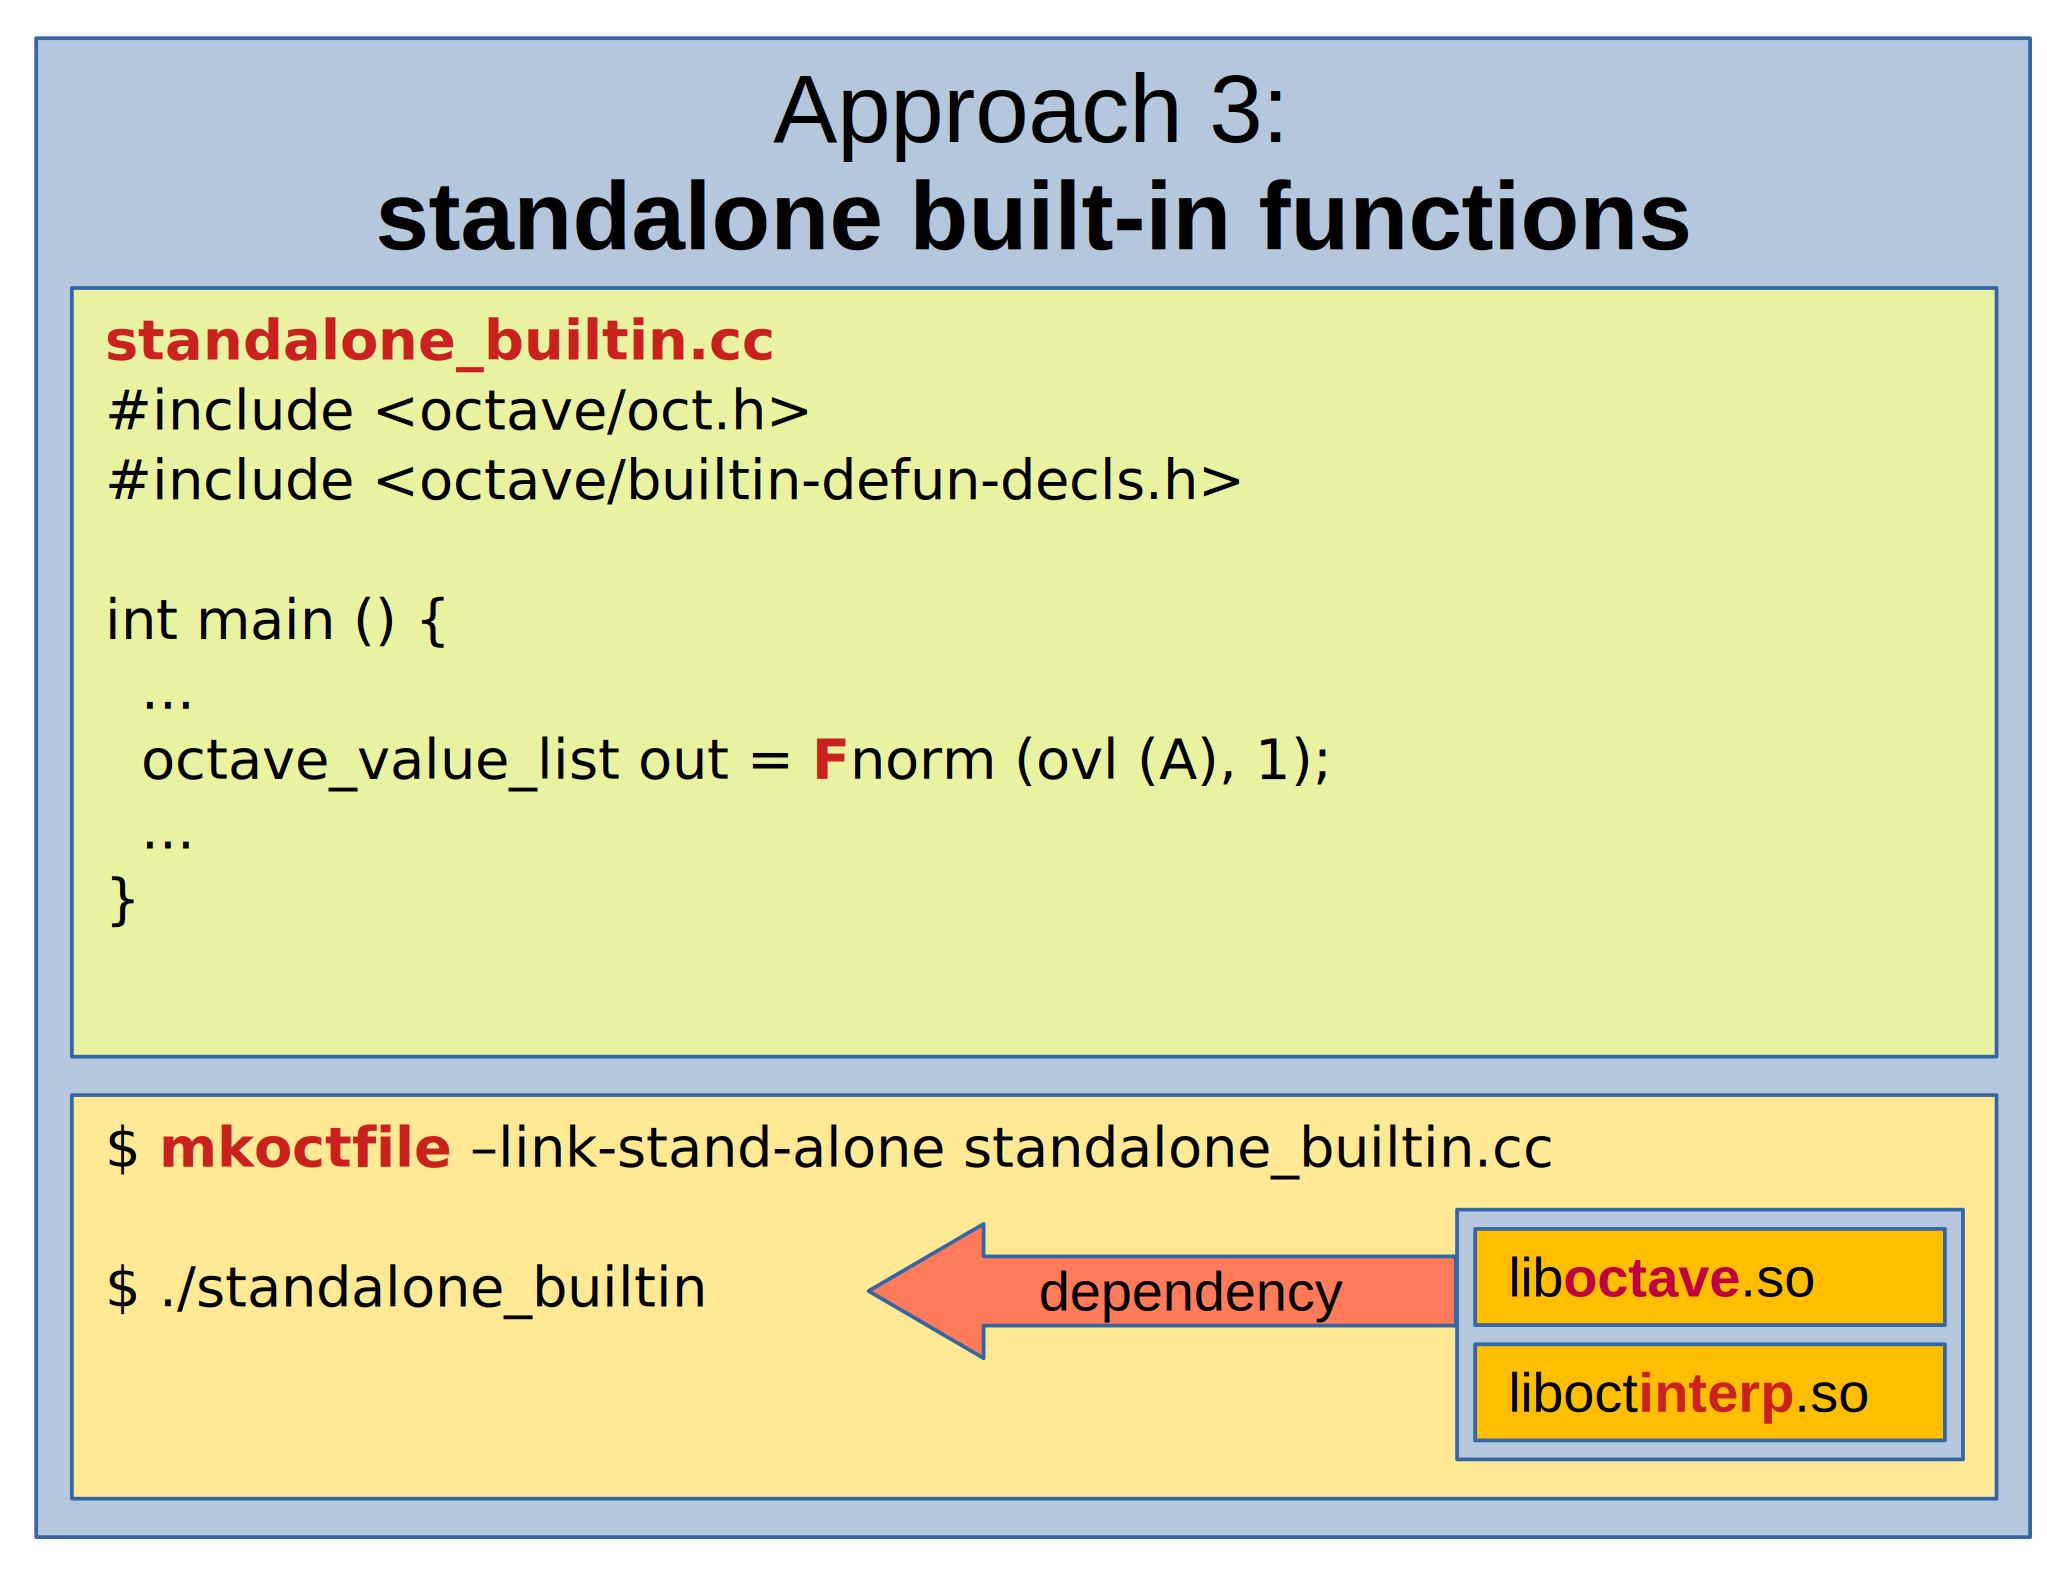
\includegraphics[width=\textwidth]{res/libreoffice/octave_c_cpp_fortran_3}
\end{column}
\begin{column}{0.3\textwidth}
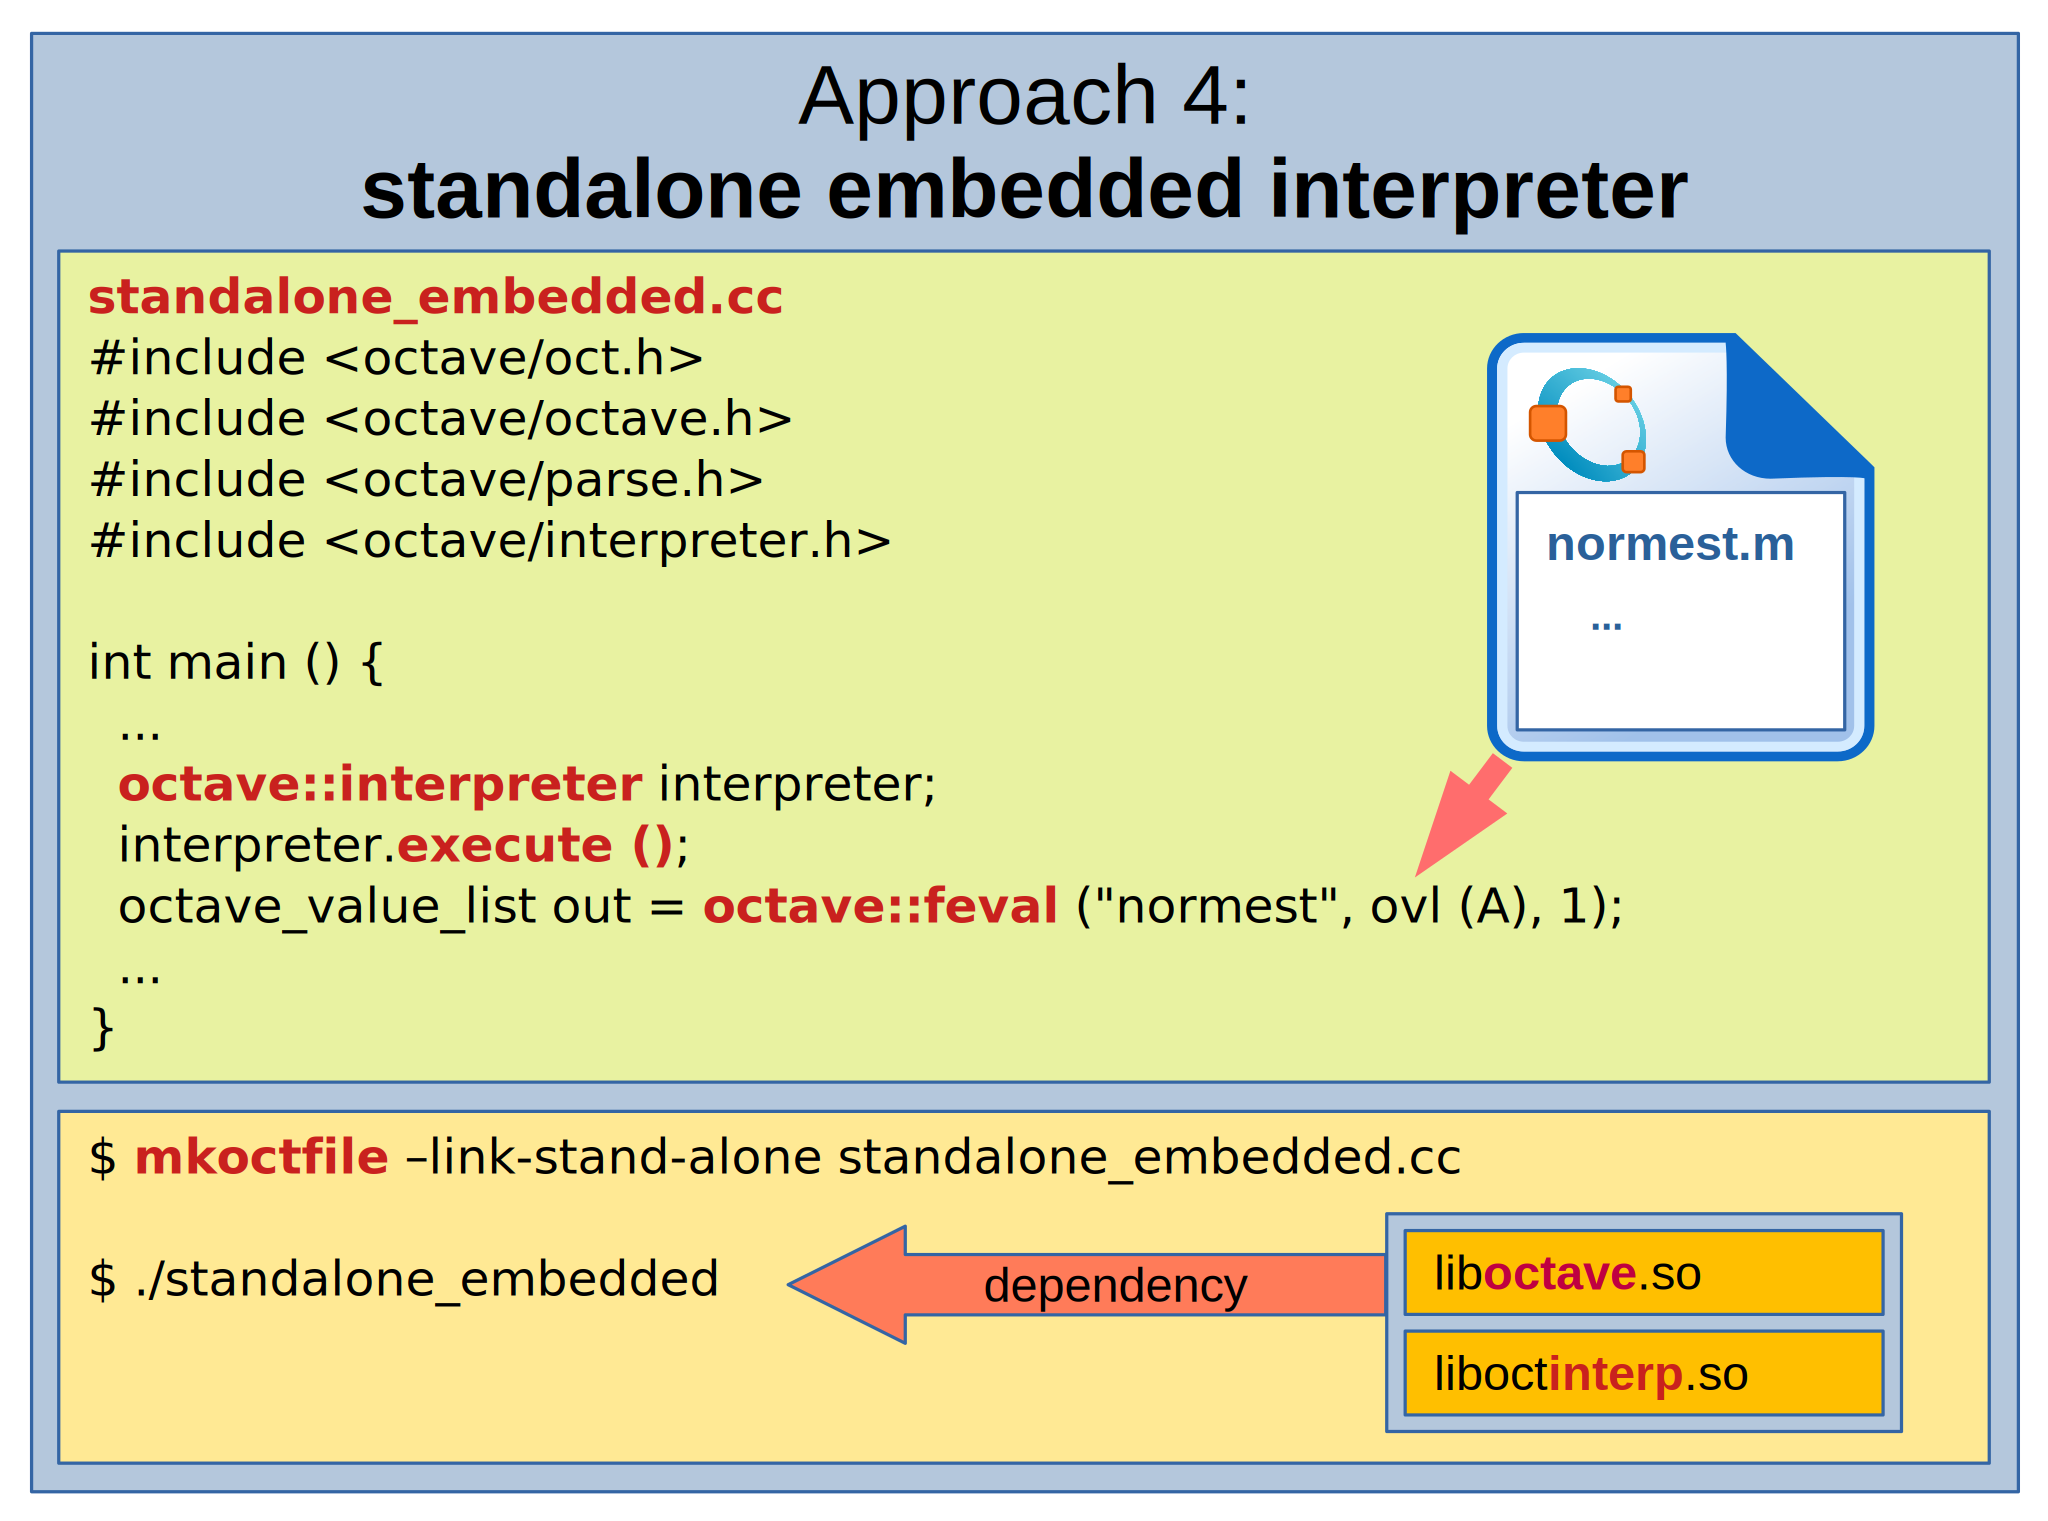
\includegraphics[width=\textwidth]{res/libreoffice/octave_c_cpp_fortran_4}
\end{column}
\end{columns}
easy \hfill difficult
\end{frame}